\PassOptionsToPackage{unicode=true}{hyperref} % options for packages loaded elsewhere
\PassOptionsToPackage{hyphens}{url}
%
\documentclass[ignorenonframetext,]{beamer}
\usepackage{pgfpages}
\setbeamertemplate{caption}[numbered]
\setbeamertemplate{caption label separator}{: }
\setbeamercolor{caption name}{fg=normal text.fg}
\beamertemplatenavigationsymbolsempty
\usepackage{lmodern}
\usepackage{amssymb,amsmath}
\usepackage{ifxetex,ifluatex}
\usepackage{fixltx2e} % provides \textsubscript
\ifnum 0\ifxetex 1\fi\ifluatex 1\fi=0 % if pdftex
  \usepackage[T1]{fontenc}
  \usepackage[utf8]{inputenc}
  \usepackage{textcomp} % provides euro and other symbols
\else % if luatex or xelatex
  \usepackage{unicode-math}
  \defaultfontfeatures{Ligatures=TeX,Scale=MatchLowercase}
\fi
\usetheme[]{Pittsburgh}
\usecolortheme{spruce}
\usefonttheme{structurebold}
% use upquote if available, for straight quotes in verbatim environments
\IfFileExists{upquote.sty}{\usepackage{upquote}}{}
% use microtype if available
\IfFileExists{microtype.sty}{%
\usepackage[]{microtype}
\UseMicrotypeSet[protrusion]{basicmath} % disable protrusion for tt fonts
}{}
\IfFileExists{parskip.sty}{%
\usepackage{parskip}
}{% else
\setlength{\parindent}{0pt}
\setlength{\parskip}{6pt plus 2pt minus 1pt}
}
\usepackage{hyperref}
\hypersetup{
            pdftitle={Far Flung Forest Landscapes in the Anthropocene},
            pdfauthor={M.K. Lau (Ph.D.)},
            pdfborder={0 0 0},
            breaklinks=true}
\urlstyle{same}  % don't use monospace font for urls
\newif\ifbibliography
% Prevent slide breaks in the middle of a paragraph:
\widowpenalties 1 10000
\raggedbottom
\setbeamertemplate{part page}{
\centering
\begin{beamercolorbox}[sep=16pt,center]{part title}
  \usebeamerfont{part title}\insertpart\par
\end{beamercolorbox}
}
\setbeamertemplate{section page}{
\centering
\begin{beamercolorbox}[sep=12pt,center]{part title}
  \usebeamerfont{section title}\insertsection\par
\end{beamercolorbox}
}
\setbeamertemplate{subsection page}{
\centering
\begin{beamercolorbox}[sep=8pt,center]{part title}
  \usebeamerfont{subsection title}\insertsubsection\par
\end{beamercolorbox}
}
\AtBeginPart{
  \frame{\partpage}
}
\AtBeginSection{
  \ifbibliography
  \else
    \frame{\sectionpage}
  \fi
}
\AtBeginSubsection{
  \frame{\subsectionpage}
}
\setlength{\emergencystretch}{3em}  % prevent overfull lines
\providecommand{\tightlist}{%
  \setlength{\itemsep}{0pt}\setlength{\parskip}{0pt}}
\setcounter{secnumdepth}{0}

% set default figure placement to htbp
\makeatletter
\def\fps@figure{htbp}
\makeatother

\usepackage{graphicx} \usepackage{tikz}

\title{Far Flung Forest Landscapes in the Anthropocene}
\providecommand{\subtitle}[1]{}
\subtitle{Structural analysis of China's embodied forest network}
\author{M.K. Lau (Ph.D.)}
\date{}

\begin{document}
\frame{\titlepage}

\begin{frame}{Overview}
\protect\hypertarget{overview}{}

\begin{itemize}
\tightlist
\item
  Intro/Context

  \begin{itemize}
  \tightlist
  \item
    Forests are globally important
  \item
    Anthropocence effects
  \item
    Global forest loss and gain and change

    \begin{itemize}
    \tightlist
    \item
      Global greening = India(Agriculture) + China(Forests)
    \end{itemize}
  \end{itemize}
\item
  Economics*Ecology = Landscape Extended Models
\item
  Network Analysis of China's Greening

  \begin{itemize}
  \tightlist
  \item
    Global Scale
  \item
    Local Scale

    \begin{itemize}
    \tightlist
    \item
      Landscape = Chen 2019
    \item
      Resilience Analysis of China's Forest LE-MRIO
    \end{itemize}
  \end{itemize}
\item
  Conclusions and Future Work
\item
  Acknowledgements
\end{itemize}

\end{frame}

\begin{frame}{Forests are Important Globally}
\protect\hypertarget{forests-are-important-globally}{}

\begin{itemize}
\tightlist
\item
  biodiversity
\item
  water and nutrient cycling
\item
  carbon storage
\item
  resources(wood, food)
\item
  culturally
\end{itemize}

\end{frame}

\begin{frame}{The Anthropocene}
\protect\hypertarget{the-anthropocene}{}

\begin{itemize}
\tightlist
\item
  Humans = dominant global impact -\textgreater{} Anthropocene
\item
  Global = Climate Change
\item
  Indirect Effects Significant
\end{itemize}

\end{frame}

\begin{frame}{In the Anthropocene, Economy is Global Ecology}
\protect\hypertarget{in-the-anthropocene-economy-is-global-ecology}{}

\begin{itemize}
\tightlist
\item
  Economic trade data is a window into human impacts
\item
  Brief history of IO and ENA analyses
\item
  Global Trade Models
\item
  Trade Networks MRIO = Sectors + Regions
\item
  Environmental Extensions
\item
  Forested Landscapes and Embodied Trade Networks
\end{itemize}

\end{frame}

\begin{frame}{Interactions/Trade = Complex Systems}
\protect\hypertarget{interactionstrade-complex-systems}{}

\begin{itemize}
\tightlist
\item
  Indirect effecs and The far reach of the city
\item
  Complex systems = many players and indirect effects matter
  (surprising)
\end{itemize}

\end{frame}

\begin{frame}{How do we study forests in this context?}
\protect\hypertarget{how-do-we-study-forests-in-this-context}{}

\end{frame}

\begin{frame}{Background: Networks are Everywhere}
\protect\hypertarget{background-networks-are-everywhere}{}

\end{frame}

\begin{frame}{Background: Networks are Everywhere}
\protect\hypertarget{background-networks-are-everywhere-1}{}

\begin{center}\includegraphics[width=0.5\linewidth]{images/resourcetrade_network} \end{center}

\end{frame}

\begin{frame}{Background: Networks are Everywhere}
\protect\hypertarget{background-networks-are-everywhere-2}{}

\begin{center}\includegraphics[width=0.5\linewidth]{images/example_network} \end{center}

\end{frame}

\begin{frame}{Background: Ecological Network Analysis}
\protect\hypertarget{background-ecological-network-analysis}{}

\begin{itemize}
\tightlist
\item
  Ecological network theory provides predictions and metrics (Lau 2017)
\item
  Systems theory provides strategies for inteventions
\item
  ENA \textless{}- Odums, MacArthur, Ulanowicz, Patten,
\item
  SNA -\textgreater{} ecological networks (Watts and Strogatz, etc.)
\item
  Structure linked to function (Donella Meadows)
\end{itemize}

\end{frame}

\begin{frame}{Research: Why Chinese Forests?}
\protect\hypertarget{research-why-chinese-forests}{}

\begin{itemize}
\tightlist
\item
  Work = Forest Land Embodied in Trade
\end{itemize}

\end{frame}

\begin{frame}{Global forest loss and gain and change}
\protect\hypertarget{global-forest-loss-and-gain-and-change}{}

\end{frame}

\begin{frame}{Global greening}
\protect\hypertarget{global-greening}{}

\end{frame}

\begin{frame}{Global greening = India(Agriculture) + China(Forests)}
\protect\hypertarget{global-greening-indiaagriculture-chinaforests}{}

\begin{itemize}
\tightlist
\item
  India is greening agriculturally
\end{itemize}

\end{frame}

\begin{frame}{Global greening = India(Agriculture) + China(Forests)}
\protect\hypertarget{global-greening-indiaagriculture-chinaforests-1}{}

\begin{itemize}
\tightlist
\item
  China is greening through reforestation
\end{itemize}

\end{frame}

\begin{frame}{A Brief History of Forest Time in China}
\protect\hypertarget{a-brief-history-of-forest-time-in-china}{}

\begin{itemize}
\tightlist
\item
  China is big and diverse (Tropical to Alpine/Boreal)
\item
  Long history of human habitation in China
\item
  Historically, two primary regions of forestry
\item
  Forest conservation impacts harvest
\item
  Flows within China and among countries globally important
\end{itemize}

\end{frame}

\begin{frame}{Research: Why Chinese Forests?}
\protect\hypertarget{research-why-chinese-forests-1}{}

\begin{center}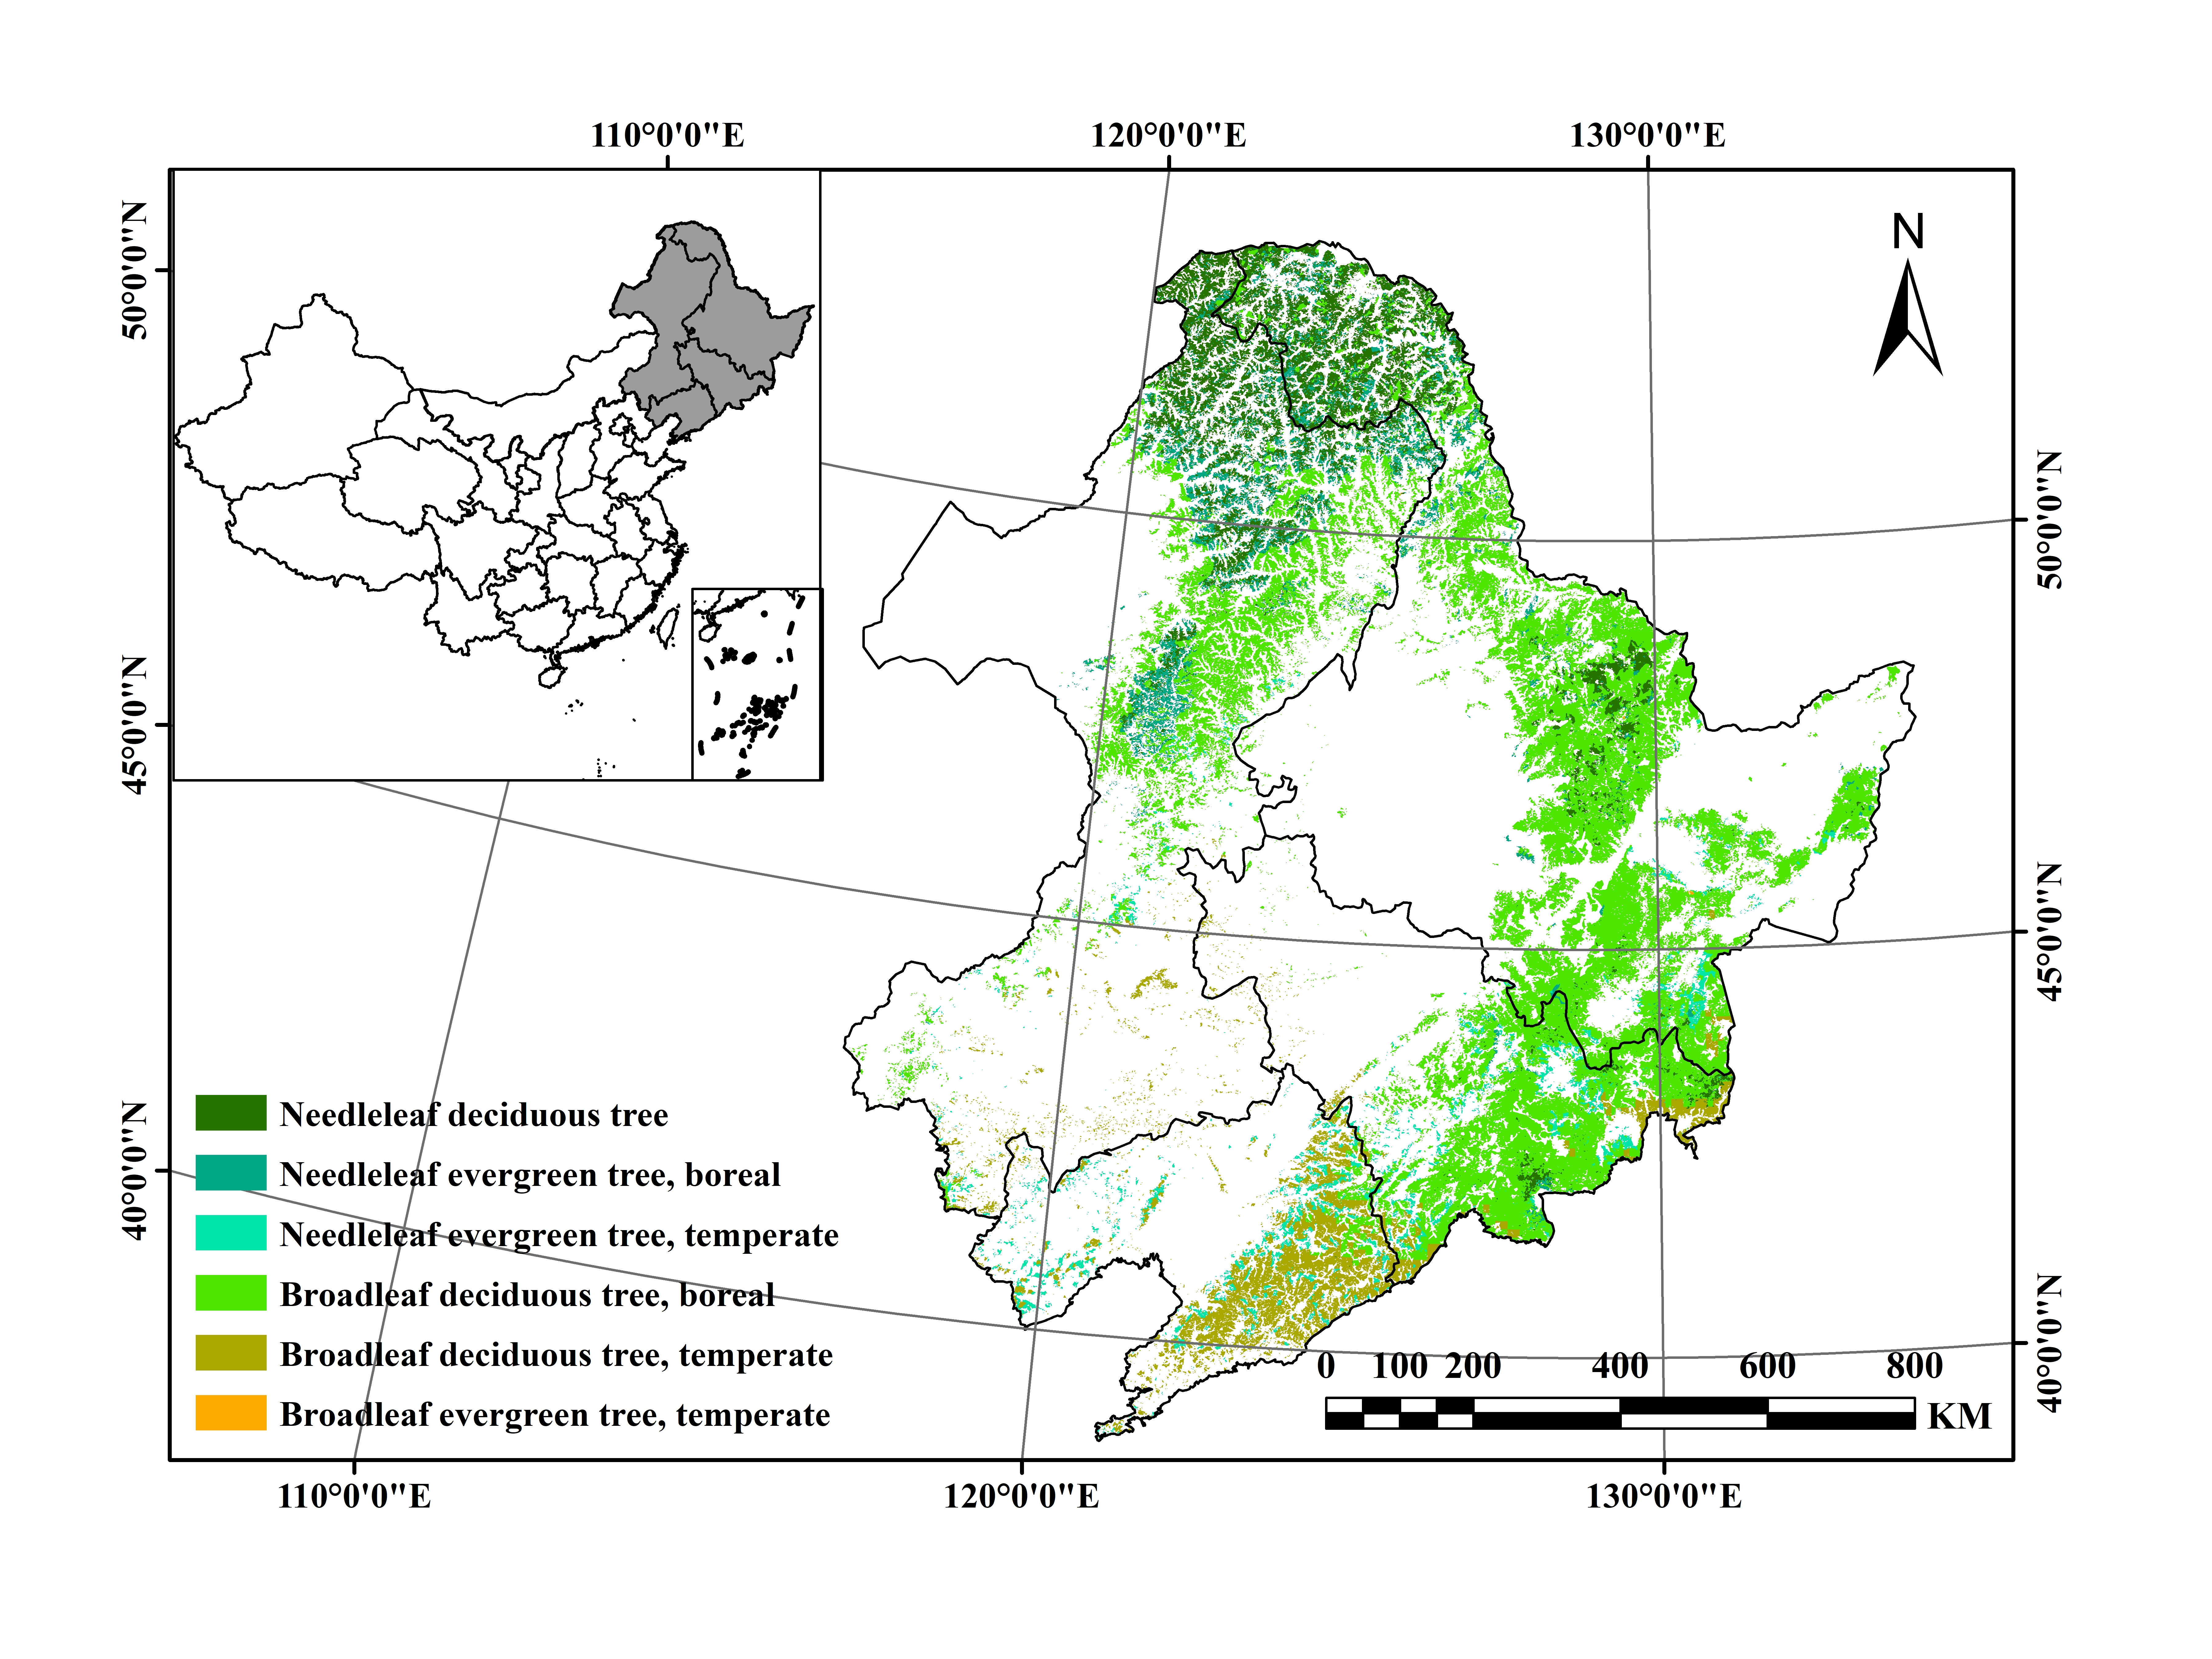
\includegraphics[width=0.5\linewidth]{images/Forest_Cover_China} \end{center}

\end{frame}

\begin{frame}{Research: Why Chinese Forests?}
\protect\hypertarget{research-why-chinese-forests-2}{}

\begin{center}\includegraphics[width=0.5\linewidth]{images/comtrade_china_imports_wood} \end{center}

\end{frame}

\begin{frame}{Network Analysis of China's Greening}
\protect\hypertarget{network-analysis-of-chinas-greening}{}

\begin{itemize}
\tightlist
\item
  Global Scale
\item
  Local Scale

  \begin{itemize}
  \tightlist
  \item
    Landscape = Chen 2019
  \item
    Resilience Analysis of China's Forest LE-MRIO
  \end{itemize}
\end{itemize}

\end{frame}

\begin{frame}{A little money moves a lot of forest.}
\protect\hypertarget{a-little-money-moves-a-lot-of-forest.}{}

\begin{itemize}
\tightlist
\item
  Tian et al.~2019 showed that China consumes an equivalent amount of
  domestic cropland as forest land, on the order of 10\(^6\) km\(^2\).
\item
  Looking at the domestic landuse productivity data for China, forests
  have the lowest monetary productivity.
\item
  Thus, per unit monetary output a relatively larger amount of forest
  land is used.
\end{itemize}

\begin{center}\includegraphics[width=0.5\linewidth]{images/Tian_2019_Fig1} \end{center}

\end{frame}

\begin{frame}{A little money moves a lot of forest.}
\protect\hypertarget{a-little-money-moves-a-lot-of-forest.-1}{}

\begin{itemize}
\tightlist
\item
  Tian et al.~2019 showed that China consumes an equivalent amount of
  domestic cropland as forest land, on the order of 10\(^6\) km\(^2\).
\item
  Looking at the domestic landuse productivity data for China, forests
  have the lowest monetary productivity.
\item
  Thus, per unit monetary output a relatively larger amount of forest
  land is used.
\end{itemize}

\begin{center}\includegraphics[width=0.5\linewidth]{images/prod_for_time_nec} \end{center}

\end{frame}

\begin{frame}{Global Landuse Trade and China}
\protect\hypertarget{global-landuse-trade-and-china}{}

\begin{center}\includegraphics[width=0.5\linewidth]{images/Tian_2019_Fig2} \end{center}

\end{frame}

\begin{frame}{Global Landuse Trade and China}
\protect\hypertarget{global-landuse-trade-and-china-1}{}

\begin{center}\includegraphics[width=0.5\linewidth]{images/Tian_2019_Fig3} \end{center}

\end{frame}

\begin{frame}{Background: Input-Output Models}
\protect\hypertarget{background-input-output-models}{}

\begin{center}\includegraphics[width=0.5\linewidth]{images/leontief_1936} \end{center}

\end{frame}

\begin{frame}{Background: Input-Output Models}
\protect\hypertarget{background-input-output-models-1}{}

\begin{itemize}
\tightlist
\item
  How do we quantify and manage systems?
\item
  Input-Output Analysis provides a modeling framework
\item
  Direct consumption
\item
  Trade occurs among sectors == Indirect consumption
\item
  IO and MRIO models
\item
  A new equation for a new era in science E = F(I-A)\^{}-1
\end{itemize}

\end{frame}

\begin{frame}{Background: Input-Output Models}
\protect\hypertarget{background-input-output-models-2}{}

\begin{center}\includegraphics[width=0.5\linewidth]{images/exiobase3} \end{center}

\end{frame}

\begin{frame}{Background: Environmental Extension}
\protect\hypertarget{background-environmental-extension}{}

\begin{itemize}
\tightlist
\item
  Allows for indirect/consumption based accounting
\end{itemize}

\begin{center}\includegraphics[width=0.5\linewidth]{images/lemrio} \end{center}

\end{frame}

\begin{frame}{Background: Environmental Extension}
\protect\hypertarget{background-environmental-extension-1}{}

\begin{center}\includegraphics[width=0.5\linewidth]{images/lemrio_equation} \end{center}

\end{frame}

\begin{frame}{wos\_mrio\_time.jpg}
\protect\hypertarget{wos_mrio_time.jpg}{}

\begin{center}\includegraphics[width=0.5\linewidth]{images/wos_mrio_time} \end{center}

\end{frame}

\begin{frame}{wos\_mrio\_auth.jpg}
\protect\hypertarget{wos_mrio_auth.jpg}{}

\begin{center}\includegraphics[width=0.5\linewidth]{images/wos_mrio_auth} \end{center}

\end{frame}

\begin{frame}{wos\_mrio\_funding.jp}
\protect\hypertarget{wos_mrio_funding.jp}{}

\begin{center}\includegraphics[width=0.5\linewidth]{images/wos_mrio_funding} \end{center}

\end{frame}

\begin{frame}{wos\_mrio\_field.jp}
\protect\hypertarget{wos_mrio_field.jp}{}

\begin{center}\includegraphics[width=0.5\linewidth]{images/wos_mrio_field} \end{center}

\end{frame}

\begin{frame}{wos\_mrio\_region.jpg}
\protect\hypertarget{wos_mrio_region.jpg}{}

\begin{center}\includegraphics[width=0.5\linewidth]{images/wos_mrio_region} \end{center}

\end{frame}

\begin{frame}{Which metric?}
\protect\hypertarget{which-metric}{}

\begin{itemize}
\tightlist
\item
  Information
\end{itemize}

\end{frame}

\begin{frame}{Why information metrics?}
\protect\hypertarget{why-information-metrics}{}

\begin{itemize}
\tightlist
\item
  Related to Shannon Information/Diversity index
\item
  \[H = -\sum_i^n p_i log(p_i)\]
\end{itemize}

\end{frame}

\begin{frame}{Methods: Model MRIO\(_{China}\)}
\protect\hypertarget{methods-model-mrio_china}{}

\begin{center}\includegraphics[width=0.5\linewidth]{images/Wu_2018_Table1} \end{center}

\end{frame}

\begin{frame}{Methods: Model MRIO\(_{China}\)}
\protect\hypertarget{methods-model-mrio_china-1}{}

\begin{center}\includegraphics[width=0.5\linewidth]{images/Wu_2018_Fig2} \end{center}

\end{frame}

\begin{frame}{Methods: Environmentally Extended Model MRIO\(_{China}\)}
\protect\hypertarget{methods-environmentally-extended-model-mrio_china}{}

\begin{center}\includegraphics[width=0.5\linewidth]{images/china_eemrio} \end{center}

\end{frame}

\begin{frame}{Methods: Model Source}
\protect\hypertarget{methods-model-source}{}

\textbf{NEED TO ADD FIGURE WITH DATA FLOWS}

\emph{Maybe check the Mi 2018 supp mat}

\begin{center}\includegraphics[width=0.5\linewidth]{images/exiobase3} \end{center}

\end{frame}

\begin{frame}{Main Focus of Research}
\protect\hypertarget{main-focus-of-research}{}

\begin{enumerate}
\tightlist
\item
  What research has been done on forest or forest landscape embodied
  networks?
\item
  What is the network structure? How can we characterize it?
\item
  What can we say about the potential system dynamics based on network
  structure?
\end{enumerate}

\end{frame}

\begin{frame}{Research: Network Analysis}
\protect\hypertarget{research-network-analysis}{}

\begin{itemize}
\tightlist
\item
  LEMRIO global (Tian 2019)
\item
  LEMRIO local (Chen 2019)
\item
  Your LE-MRIO China
\item
  Your ENA analysis

  \begin{itemize}
  \tightlist
  \item
    Small world
  \item
    Modularity
  \item
    Centrality
  \item
    Control
  \item
    Resilience
  \end{itemize}
\end{itemize}

\end{frame}

\begin{frame}{Research: Structural Analysis}
\protect\hypertarget{research-structural-analysis}{}

\begin{itemize}
\tightlist
\item
  Analysis = Structure = Robustness
\end{itemize}

\begin{center}\includegraphics[width=0.5\linewidth]{images/Fath_2015_Fig6} \end{center}

\end{frame}

\begin{frame}{Research: Structural Analysis}
\protect\hypertarget{research-structural-analysis-1}{}

\begin{itemize}
\tightlist
\item
  Overly efficient = Brittle
\item
  Overly redundant = Stagnant
\item
  Both can lead to niche opennings
\item
  Niches can then be filled by natural selection, adaptation or invasion
\end{itemize}

\end{frame}

\begin{frame}{Forest Landscape Networks are More Efficient but Less
Robust}
\protect\hypertarget{forest-landscape-networks-are-more-efficient-but-less-robust}{}

\begin{center}\includegraphics[width=0.5\linewidth]{images/for-rob-red} \end{center}

\end{frame}

\begin{frame}{Caveats}
\protect\hypertarget{caveats}{}

\begin{itemize}
\tightlist
\item
  Limitations of MRIO
\item
  Potential impacts of storage lags and buffers
\end{itemize}

\end{frame}

\begin{frame}{Future: Next up, climate change variability}
\protect\hypertarget{future-next-up-climate-change-variability}{}

\begin{itemize}
\tightlist
\item
  Next up = Climate change impacts and global scale
\end{itemize}

\begin{center}\includegraphics[width=0.5\linewidth]{images/lemrio_climate_change} \end{center}

\end{frame}

\begin{frame}{Future: Next up, climate change variability}
\protect\hypertarget{future-next-up-climate-change-variability-1}{}

\begin{center}\includegraphics[width=0.1\linewidth]{images/lemrio_climate_workflow} \end{center}

\end{frame}

\begin{frame}{Future Work: Remote Sensing Trade Models}
\protect\hypertarget{future-work-remote-sensing-trade-models}{}

\begin{center}\includegraphics[width=0.1\linewidth]{images/Moran_2020_Fig1} \end{center}

\end{frame}

\begin{frame}{Q \& A}
\protect\hypertarget{q-a}{}

\end{frame}

\end{document}
